\section{\label{appendix:JAX}JAX NumPy: Usage Tutorial}

JAX is a Python library developed by Google that provides an easy and efficient way to perform numerical computations, particularly those involving large matrices and tensors, on a GPU. JAX uses a technique called \textit{Just-In-Time (JIT) compilation}, which compiles the Python code into optimized machine code that can run on the GPU. This allows JAX to take advantage of the parallelism offered by the GPU, making computations much faster than if they were performed on the CPU.

One of the key features of JAX is its ability to automatically differentiate functions. JAX also provides a set of linear algebra operations that are optimized for GPU acceleration, including matrix multiplication, matrix-vector multiplication, and matrix inversion. To perform matrix operations using JAX, one first needs to create arrays or tensors that contain the matrix data and then use the JAX linear algebra functions to perform matrix operations on these arrays. 

The usage of the JAX NumPy library involves a minor change in standard NumPy Python code by replacing most NumPy function calls with JAX NumPy calls. For example, to define a 2-D tensor of zeroes of shape $(5,3)$ in JAX NumPy, we would do the following:

\begin{verbatim}
    import jax.numpy as jnp
    new_arr = jnp.zeros((5,3))
\end{verbatim}

To use the JIT feature of JAX NumPy, we can think of JIT as a decorator that accepts functions operating on JAX arrays and their arguments as static arguments. For example, if we have a function 'addJAX' defined over JAX NumPy arrays, we would tell the Python interpreter to use JIT compilation for this function as follows:

\begin{verbatim}
    from jax import jit
    add_jit = jit(addJAX)
\end{verbatim}

JAX NumPy does not allow tensor slicing or direct indexing but rather makes use of the C++ style `at' function to access tensor elements by index. In addition, JAX tensors are immutable, i.e. they cannot be edited in place. Please refer to the official documentation of JAX NumPy for further details on JAX methods at \url{https://jax.readthedocs.io/en/latest/jax.numpy.html}


\section{\label{appendix:GPU-acc-comparison}Comparison of different off-the-shelf GPU-based tensor manipulation libraries}

For the centralized joint trajectory optimization problem for multiple holonomic robots, we implement the path planning algorithm using three different off-the-shelf open-source Python libraries - vanilla NumPy, JAX NumPy and CuPy. The latter two libraries use accelerated tensor computations to achieve computational speed-up in computing large tensor operations, such as matrix multiplications, inverses, and so on. As discussed in Appendix \ref{appendix:JAX}, JAX NumPy leverages GPU acceleration for CUDA-based tensor computations, and so does CuPy. Table \ref{table: gpu-acc-comp} compares the time taken to plan start-to-goal offline trajectories for a varying number of robots using the same core centralized trajectory optimization approach.

\begin{table}
\centering
\caption{Comparison of planning times using different mathematical libraries} \label{table: gpu-acc-comp}
\scriptsize
\begin{tabular}{|p{3cm}|p{3cm}|p{3cm}|}\hline
 Number of Robots & Planning time(in sec) & Library
\\ \hline
4 & 0.0050 & NumPy
\\ \hline
8 & 0.0049 & NumPy
\\ \hline
16 & 0.0046 & CuPy
\\ \hline
32 & 0.0046 & JAX NumPy
\\ \hline
32 & 0.267 & NumPy
\\ \hline
32 & 0.0049 & CuPy
\\ \hline
64 & 0.0047 & JAX NumPy
\\ \hline
\end{tabular}
\normalsize
\vspace{-0.7cm}
\end{table}

We observe from Table \ref{table: gpu-acc-comp} that compared to NumPy, JAX NumPy achieves a computational acceleration of around $60$ times over vanilla NumPy by leveraging GPU computations. Further, the planning time for 32 as well as 64 robots are similar, indicating that the JAX-based implementation of the algorithm remains nearly constant regardless of the increase in the number of robots, or, in other words, an increase in the size of the matrices used in the optimization process. For CuPy, we observe a similar trend in the planning time, where between 16 and 32 robots, the computation time remains nearly constant as well. 

\section{Initializations using Reciprocal Velocity Obstacle(RVO)\cite{RVO}}\label{sec:appendix-RVO}

RVO is a local, reactive multi-robot trajectory planner that has been shown to generate collision-free trajectories in real-time for hundreds of Robots\cite{RVO}. Even though it runs in real-time, RVO trajectories cannot be directly executed by Robots as they are jittery and jerky. We use a trick to precompute trajectories using RVO for given start and goal positions of multiple Robots and use the RVO trajectories along with other optimizer parameters computed from them to initialize our optimizer. Thus the task of eliminating collisions is first performed by RVO and further enhanced by our optimizer. We consider the velocity along the straight line joining the start and goal positions of the Robots as the desired velocity in RVO and sample the RVO trajectory obtained at evenly spaced intervals to match the number of time samples expected by the optimizer. We define the following set of additional configurations to test our optimizer with different types of initializations:

\begin{itemize}
  \item \textbf{Square Antipodal:}
  Robots are placed on the edge of a square and are needed to reach their antipodal positions. This scenario is particularly challenging since if the robots were moving in straight lines between the start and goal positions, they would all collide together at the center of the workspace.
  \item \textbf{Circle:}
  Robots are distributed evenly along a circle and are needed to rotate by $k$ positions. (default $k=5$).
  \item \textbf{Ellipse:}
  Robots are placed uniformly along a straight line, and the $i^{th}$ robot is needed to reach the position of the $(n-i)^{th}$ robot where $n$ is the total number of robots.
\end{itemize}

Figure \ref{fig:RVO+opti_2D} shows the trajectories generated by RVO alone for 16 Robots in the Square Antipodal scenario vs trajectories generated by our optimizer with RVO initialization. We observe a significant improvement in the smoothness of the trajectories generated by our optimizer with RVO initialization compared to RVO alone. The improvement in trajectory quality can be explained as follows: the optimizer starts with an already low residual due to RVO initialization and further reduces it with iterations while smoothing the trajectories at the same time. However, in terms of computation time, the RVO initialization does not offer significant benefits compared to a straight-line initialization of trajectories. 

\begin{figure}[H]
    \centering
    {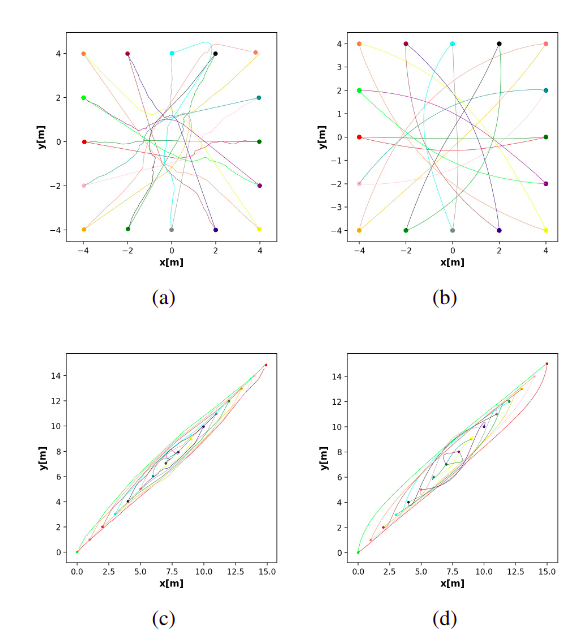
\includegraphics[scale=0.6]{figures/appendix/RVO_inits.png}} 
    \caption[Appendix: Trajectories using RVO + multirobot optimizer]{Comparison of trajectories from a) RVO alone in 16 Robots 2D Square Antipodal b) Optimizer + RVO initialization for 16 Robots 2D Square Antipodal c) RVO alone in 16 Robots 2D Ellipse b) Optimizer + RVO initialization for 16 Robots 2D Ellipse.}
    \label{fig:RVO+opti_2D}
\end{figure}

\section{Initializations using Multi-robot Pathfinding(MAPF)\cite{sharon_journal}}\label{sec:appendix-MAPF}

Similar to RVO, we can also couple graph-search-based Multi-robot Pathfinding (MAPF) algorithms discussed in Section \ref{sec:MAPF} for initializing our optimizer. For this purpose, we will use the \texttt{cbs-mapf} PyPI package that implements the high-level Conflict Based Search Algorithm based on \cite{sharon_journal} and low-level space-time A*(STA*), which is similar to normal A*(from Section \ref{sec:A*} with an additional time dimension. The trajectories generated by CBS-MAPF are piecewise linear and exhibit jerks and sharp turns, so these cannot be used practically for multi-robot navigation. We scale up the start and goal coordinates depending on grid size (we use grid size = 10) as well as the robot radii and precompute multirobot trajectories using CBS-MAPF. Similar to the RVO trajectories, we sample points from the trajectories obtained from CBS-MAPF to calculate the optimizer parameters and initialize our optimizer. 

We introduce a new scenario to test MAPF for 14 Robots arranged in a 2D grid and are needed to move to the opposite end of the grid. Figure \ref{fig:MAPF+opti_grid} shows a comparison of trajectories between CBS-MAPF alone and the optimizer using CBS-MAPF for initialization. We again observe a significant improvement in the smoothness of the trajectories generated by our optimizer with CBS-MAPF initialization compared to CBS-MAPF alone. However, similar to RVO, there is no benefit to using MAPF initialization in terms of computational time. 

\begin{figure}[H]
    \centering
    {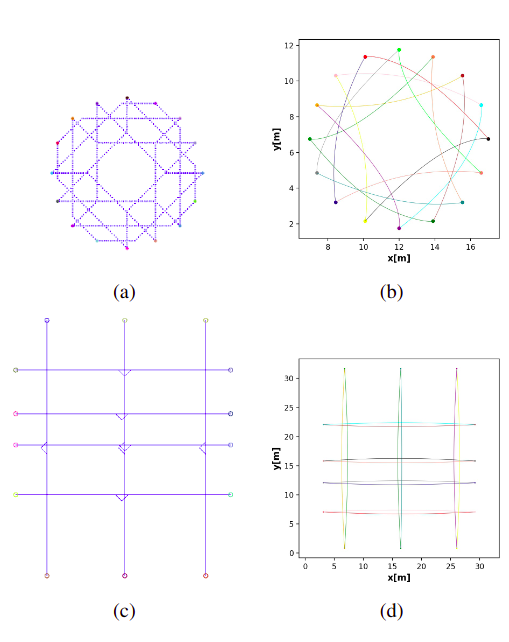
\includegraphics[scale=0.6]{figures/appendix/mapf_init.png}} 
    \caption[Appendix: Trajectories using MAPF + multirobot optimizer]{Comparison of trajectories generated by CBS-MAPF alone and our optimizer with CBS-MAPF initialization for a)-b) 16 Robots in the Circle(k=5) scenario, c)-d) 14 Robots in 2D Grid orientation.}
    \label{fig:MAPF+opti_grid}
\end{figure}